
\chapter{Buffers, Windows and Frames}
\label{cha:buff-wind-fram}

\section{Concepts}
\label{sec:concepts}
\begin{figure}[H]
  \centering
  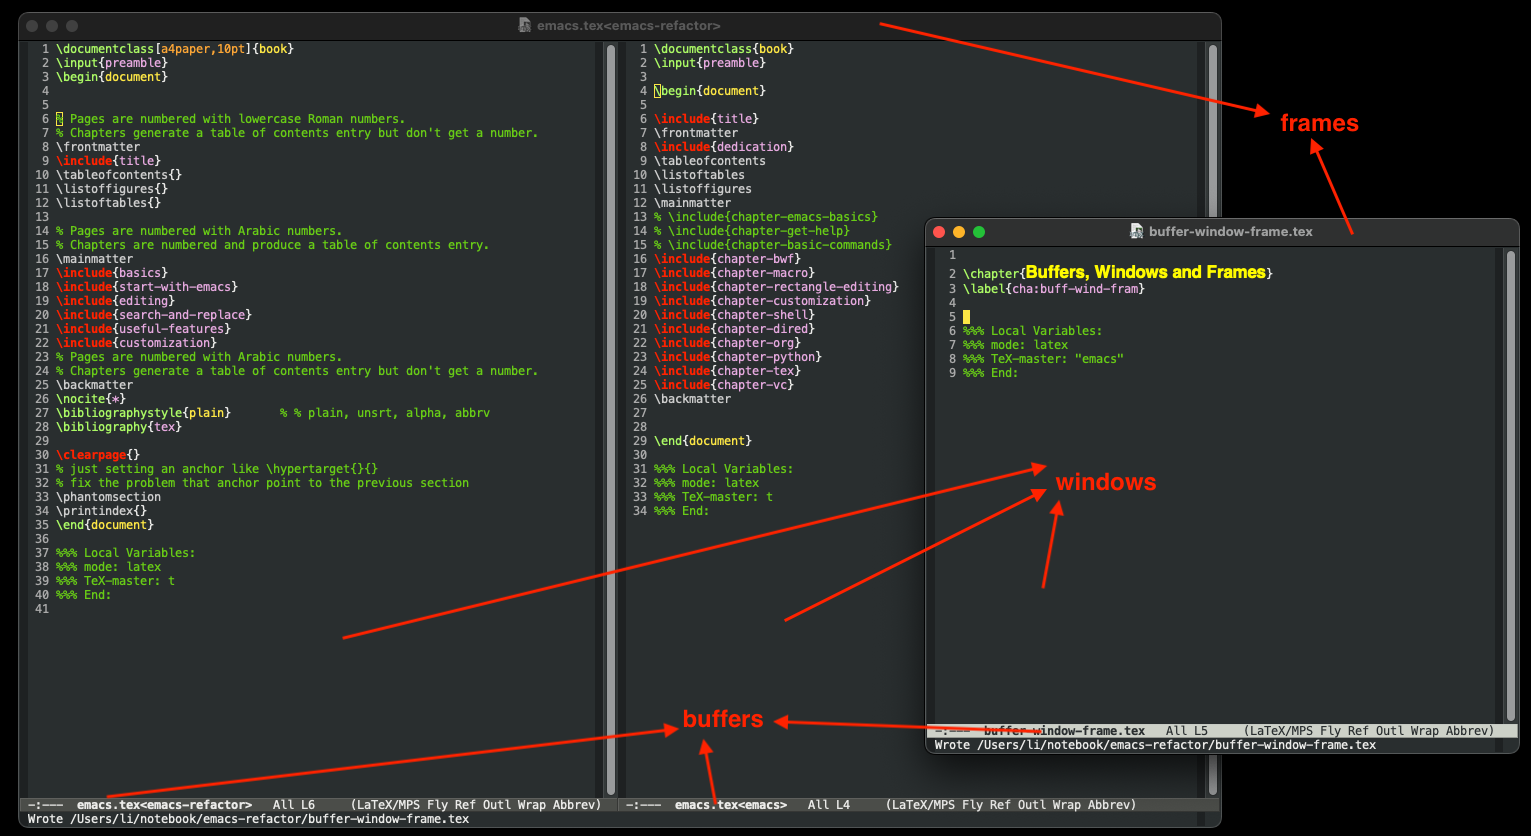
\includegraphics[width=0.9\textwidth]{bwf}  
  \caption{Buffers, windows and frames}
  \label{fig:bwf}
\end{figure}


Buffers are independent of windows and frames.
A Buffer may contains a file or be Emacs-generated.
The name of the buffer that containing a file is the same name with the file.
The name of the buffer that are Emacs-generated has the format \argument{*buffer name*}.
For example, \argument{*Help*, *scratch*, *Messages*} as so on.

\newpage{}
\section{Buffer Commands}
\label{sec:buffer-commands}

\begin{table}[H]
  \centering
  \begin{tabular}{>{\bfseries}ll}
    \toprule
    \head{Binding} & \head{Meaning}\\
    \midrule
    C-x b & move to most recently buffer or the specified buffer\\
    C-x k & delete buffer\\
    C-x C-s & save buffer\\
    C-x s & save all buffers\\
    C-x C-q & toggle read only mode\\
    C-x C-b & list all buffers\\
    \bottomrule
  \end{tabular}
  \caption{Buffer Commands}
  \label{tab:buffer-commands}
\end{table}


\subsection{Buffer List}
\label{sec:buffer-list}

\keyword{C-x C-b} creates a new \argument{*Buffer List*} window on the screen.
It is shown in the following Figure \ref{fig:buffer-list}.
The \argument{CRM} column has the following available values:
\begin{itemize}
\item \keyword{.} : displayed 
\item \keyword{*} : modified
\item \keyword{\%} : read only
\item \keyword{D} : marked for deletion
\item \keyword{>} : marked for display
\item \keyword{S} : marked for saving
\end{itemize}

\begin{figure}[H]
  \centering
  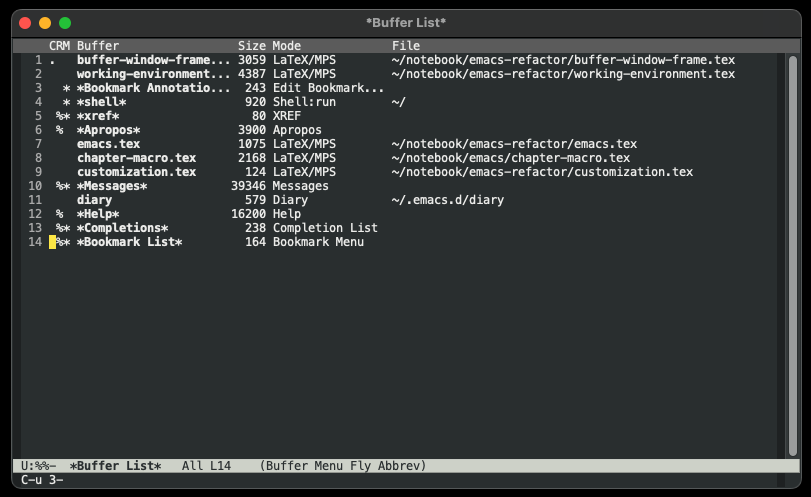
\includegraphics[width=0.9\textwidth]{buffer-list}
  \caption{Buffer list}
  \label{fig:buffer-list}
\end{figure}

\begin{table}[H]
  \centering
  \begin{tabular}{>{\bfseries}ll}
    \toprule
    \head{Keystroke} & \head{Meaning}\\
    \midrule
    C-n or n & down one line\\
    C-p or p & up one line\\
    \midrule
    m & mark buffer to be displayed\\
    d & mark buffer for deletion\\
    s & mark buffer for save\\
    u & unmark buffer\\
    U & remove all marks from all lines\\
    Del & unmark the previous buffer, if there is no mark, move up one line\\
    \midrule
    x & execute other one-letter commands on all marked buffers\\
    v & display buffers marked with \argument{m}\\
    \midrule
    T & toggle whether the menu displays only file buffers\\
    \% & toggle read-only status of buffer\\
    \midrule
    RET & select current line's buffer in place of the buffer menu\\
    V & select current line’s buffer, in View mode\\
    1 & display buffer in a full screen\\
    2 & display this buffer and the next one in horizontal windows\\
    f & replace buffer list with this buffer\\
    o & replace other window with this buffer\\
    C-o & make another window display that buffer\\
    t & visit the tags table in the buffer on this line.\\
    \midrule
    M-s a C-s & incremental search in the marked buffers\\
    M-s a C-M-s & isearch for regexp in the marked buffers\\
    \midrule
    q & quit buffer list\\
    \bottomrule
  \end{tabular}
  \caption{Buffer list commands}
  \label{tab:buffer-list-commands}
\end{table}



\section{Window Commands}
\label{sec:window-commands}

\begin{table}[H]
  \centering
  \begin{tabular}{>{\bfseries}ll}
    \toprule
    \head{Binding} & \head{Meaning}\\
    \midrule
    C-x o & switch to other window\\
    C-x 0 & delete current window\\
    C-x 1 & delete other windows\\
    C-x 2 & split window down\\
    C-x 3 & split window right\\
    \midrule
    C-x \textasciicircum{} & enlarge window vertically\\
    C-x \} & enlarge window horizontally\\
    C-x \{ & shrink window horizontally\\
    \midrule
    C-x - & shrink window if larger than buffer\\
    C-x + & balance window\\
    \bottomrule
  \end{tabular}
  \caption{Window Commands}
  \label{tab:window-commands}
\end{table}

A number of the ``other window'' commands are just the ordinary command with a 4 inserted in it.
For example, to find a file in another window, type \keyword{C-x 4 f}.
To select a different buffer in another window, type \keyword{C-x 4 b}.
These commands save you steps: you do not need move to the other window, give a command and move back.

\subsection{Package "ace-window"}
\label{sec:package-ace-window}

Using \keyword{C-x o} to switch between windows if there are only two windows.
It quickly loses its value when there are more windows.
``ace-window'' is used to solve this problem.
\begin{lstlisting}[language=elisp]
;; Rebind M-o to ace-window
(global-set-key (kbd "M-o") 'ace-window)

;; This is the list of initial characters used in window labels.
;; The characters are used after ace-window command to select the window.
(setq aw-keys '(?a ?s ?d ?f ?g ?h ?j ?k ?l))
\end{lstlisting}

You can swap current window and a specified by calling \keyword{M-o} with a prefix argument \keyword{C-u}.
You can delete the selected window by calling \keyword{ace-window} with a double prefix argument \keyword{C-u C-u}.




\section{Frame Commands}
\label{sec:frame-commands}

\begin{table}[H]
  \centering
  \begin{tabular}{>{\bfseries}ll}
    \toprule
    \head{Binding} & \head{Meaning}\\
    \midrule
    C-x 5 o & switch to other frame\\
    C-x 5 0 & delete current frame\\
    C-x 5 1 & delete other frame\\
    C-x 5 2 & create a new frame on the current buffer\\
    \bottomrule
  \end{tabular}
  \caption{Frame Commands}
  \label{tab:frame-commands}
\end{table}

A number of the ``other frame'' commands are just the ordinary command with a 5 inserted in it.
For example, to find a file in another frame, type \keyword{C-x 5 f}.
To select a different buffer in another frame, type \keyword{C-x 5 b}.
These commands save you steps: you do not need move to the frame, give a command and move back.

%%% Local Variables:
%%% mode: latex
%%% TeX-master: "emacs"
%%% End:
